%%%%%%%%%%%%
%%%%%%%%%%%%
\begin{figure}
\centering
%%%%%%%%%%%%
\pgfdeclarelayer{background}
\pgfsetlayers{background,main}
%%%%%%%%%%%%
%%%%%%%%%%%%

\begin{subfigure}[t]{.22\textwidth}
	\centering
	\fbox{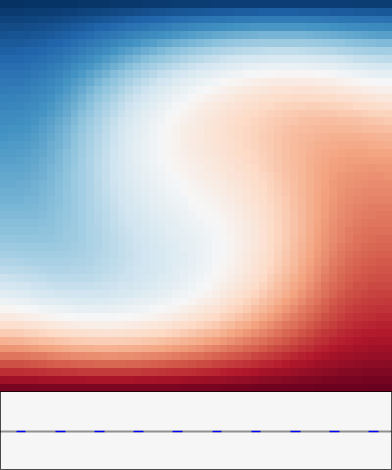
\includegraphics[width=\textwidth]{fig/rayleigh/t0.png}}
    	\caption{Initial state}
	\label{fig:rayleigh_field_0}
\end{subfigure} \quad
\begin{subfigure}[t]{.22\textwidth}
	\centering
	\fbox{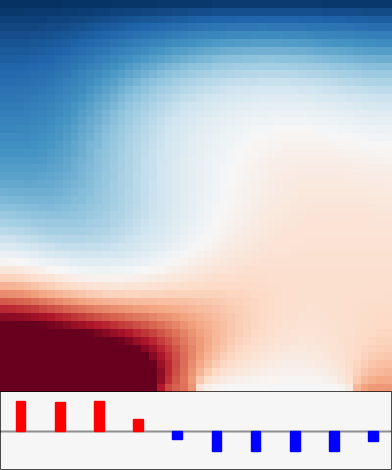
\includegraphics[width=\textwidth]{fig/rayleigh/t2.png}}
    	\caption{$t=2$}
	\label{fig:rayleigh_field_2}
\end{subfigure} \quad
\begin{subfigure}[t]{.22\textwidth}
	\centering
	\fbox{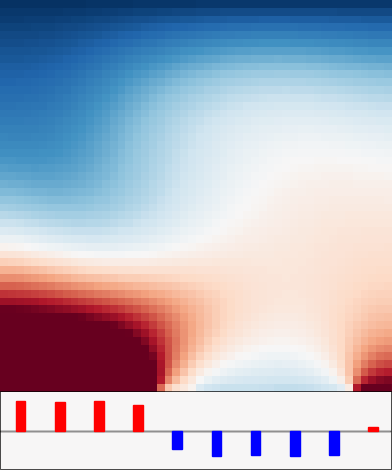
\includegraphics[width=\textwidth]{fig/rayleigh/t4.png}}
    	\caption{$t=4$}
	\label{fig:rayleigh_field_4}
\end{subfigure} \quad
\begin{subfigure}[t]{.22\textwidth}
	\centering
	\fbox{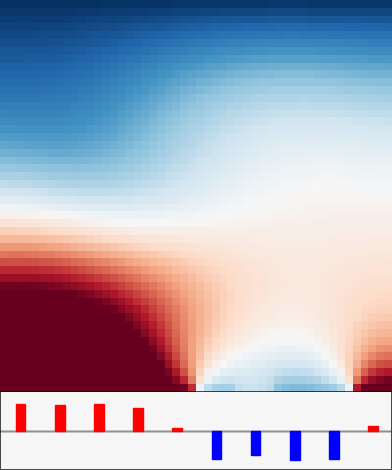
\includegraphics[width=\textwidth]{fig/rayleigh/t6.png}}
    	\caption{$t=6$}
	\label{fig:rayleigh_field_6}
\end{subfigure}

\medskip

\begin{subfigure}[t]{.22\textwidth}
	\centering
	\fbox{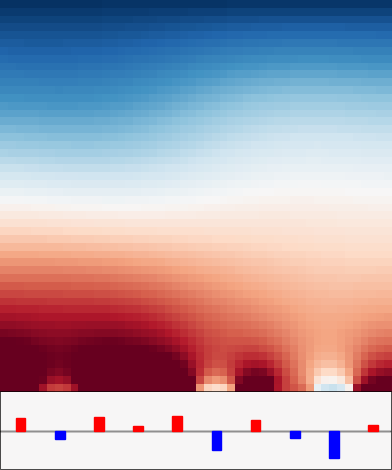
\includegraphics[width=\textwidth]{fig/rayleigh/t8.png}}
    	\caption{$t=8$}
	\label{fig:rayleigh_field_8}
\end{subfigure} \quad
\begin{subfigure}[t]{.22\textwidth}
	\centering
	\fbox{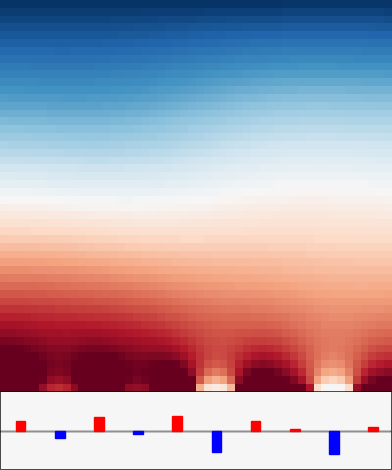
\includegraphics[width=\textwidth]{fig/rayleigh/t10.png}}
    	\caption{$t=10$}
	\label{fig:rayleigh_field_10}
\end{subfigure} \quad
\begin{subfigure}[t]{.22\textwidth}
	\centering
	\fbox{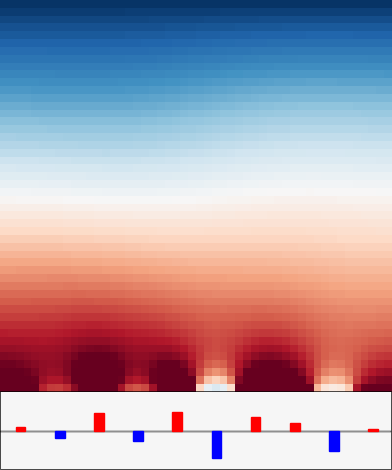
\includegraphics[width=\textwidth]{fig/rayleigh/t12.png}}
    	\caption{$t=12$}
	\label{fig:rayleigh_field_12}
\end{subfigure} \quad
\begin{subfigure}[t]{.22\textwidth}
	\centering
	\fbox{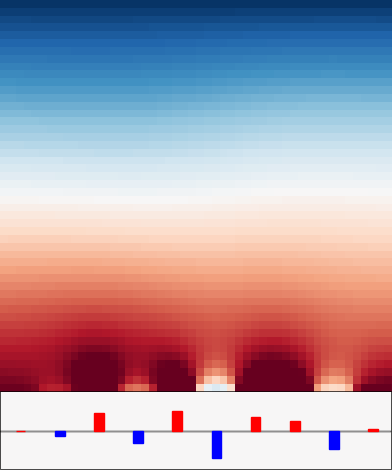
\includegraphics[width=\textwidth]{fig/rayleigh/t14.png}}
    	\caption{$t=14$}
	\label{fig:rayleigh_field_14}
\end{subfigure}

%%%%%%%%%%%%
\caption{\textbf{Evolution of the convection cell under control of the agent,} during the first steps of the environment. After a strong initial forcing, the agent establishes a pattern of alternating hot and cold actions that leads to a stationary configuration with $\nus(t) = 1$. The control of the agent remains the same for the rest of the environment.}
\label{fig:rayleigh_fields}
\end{figure} 
%%%%%%%%%%%%
%%%%%%%%%%%%